\section{embeddings}
一个embedding是一个从离散对象像字映射为一个真实值的向量,例如一个英文字符的300维的embedding可能包括:
\begin{python}
blue:  (0.01359, 0.00075997, 0.24608, ..., -0.2524, 1.0048, 0.06259)
blues:  (0.01396, 0.11887, -0.48963, ..., 0.033483, -0.10007, 0.1158)
orange:  (-0.24776, -0.12359, 0.20986, ..., 0.079717, 0.23865, -0.014213)
oranges:  (-0.35609, 0.21854, 0.080944, ..., -0.35413, 0.38511, -0.070976)
\end{python}
embedding让你能在离散的数据上应用机器学习,分类器,更常用的神经网络都被设计为一个高密度的连续向量(所有的值都用来定义一个对象)如果离散对象被编码为一个离散的院子,入独一无二的id号,他们阻止学习和泛化一种考虑embeddings的方法是转化费响亮的对象为有用的机器学习输入。,embeding作为机器学习的输出也是有用的,因为embedding映射独享为向量,在向量空间中的应用是类似的。一个通常的用法是找到一个最接近的邻居。用和相面相同的word embedding,例如对于每个字和相关的角度这里有三个接近的邻居:
\begin{python}
blue:  (red, 47.6°), (yellow, 51.9°), (purple, 52.4°)
blues:  (jazz, 53.3°), (folk, 59.1°), (bluegrass, 60.6°)
orange:  (yellow, 53.5°), (colored, 58.0°), (bright, 59.9°)
oranges:  (apples, 45.3°), (lemons, 48.3°), (mangoes, 50.4°)
\end{python}
这将告诉程序苹果和橙子类似度($45.3^o$)比柠檬和橙子($48.3^o$)更类似。
\subsection{训练一个embedding}
为了在TensorFlow中训练word embedding,首先你需要分隔文字成单词赋值给词汇表中的每一个单词一个整数。假设我们已经做了这步,word\_ids是一个整数向量。例如句子"I have a cat."可能被分割成["I","have","a","cat","."]然后相关的word\_ids tensor形状为[5]由5个整数组成。为了得到这些单词ids embeded,我们需要用tf.gather函数按照下面创建embedding变量。
\begin{python}
word_embeddings = tf.get_variable(“word_embeddings”,
    [vocabulary_size, embedding_size])
embedded_word_ids = tf.gather(word_embeddings, word_ids)
\end{python}
在这之后tensor embedded\_word\_ids在我们的例子中将有形状[5,embedding\_size]同时包含5个单词的embeddings(dese vector)。变量word\_embeddings将被学习在训练结束后它将包含所有在词汇表中的embeddings.embeddings可能被多种方式训练,依靠数据变量。例如可以用循环神经网络从语料中的句子的前一个单词预测下一个单词或者用两个网络做多种语言的翻译。这个方法在\textbf{字词的向量表示}中有描述,但是上面的所有情况下有一个像上面的embedding变量和用tf.gather的embbedded word。
\subsection{可视化Embeddings}
TensorBoard有一个内建的可视化器,称为EmbeddingProjector,用于交互式的embedding可视化。embedding projector将从你的checkpointer文件读取embeddings用PCA映射他们到3维空间。对于PCA的可视化查看\href{http://setosa.io/ev/principal-component-analysis/}{这里},另一个有用的映射是t-SNE。如果你正在embedding上工作,你可能像添加labels/images到数据点。你可以通过生成一个包含每个点的labels和用我们的Python API映射器的配置\href{https://www.tensorflow.org/programmers_guide/embedding#metadata}{metadata file},或者在和你的checkpoint文件相同多个目录手动构造和保存一个projector\_config.pbtxt。
\subsection{创建}
\begin{enumerate}
	\item 设置一个2维tensor保存你的embedding。
		\begin{python}
			embedding\_var = tf.get\_variable(...)
		\end{python}
	\item 定期保存你模型的变量到LOG\_DIR目录中
		\begin{python}
			saver = tf.train.Saver()
			saver.save(session,os.path.join(LOG_DIR,"model.ckpt"),step)
		\end{python}
	\item 结合meta data和你的embedding(可选)
\end{enumerate}
如果你有任何的metadata(labels,images)结合你的embedding,你可以调用TensorBoard通过制定存储在LOG\_DIR中的一个projector\_config.pgtxt或者用你自己的PythonAPI。例如下面的projector\_config.pbtxt结合word\_embedding tensor和存储在\$LOG\_DIR/metadata.tsv的metadata文件。
\begin{python}
embeddings {
	  tensor_name: 'word_embedding'
	    metadata_path: '$LOG_DIR/metadata.tsv'
	   }
\end{python}
相同的配置可以通过下面的代码段一程序产生:
\begin{python}
from tensorflow.contrib.tensorboard.plugins import projector
# Create randomly initialized embedding weights which will be trained.
vocabulary_size = 10000
embedding_size = 200
embedding_var = tf.get_variable('word_embedding', [vocabulary_size, embedding_size])
# Format: tensorflow/tensorboard/plugins/projector/projector_config.proto
config = projector.ProjectorConfig()
# You can add multiple embeddings. Here we add only one.
embedding = config.embeddings.add()
embedding.tensor_name = embedding_var.name
# Link this tensor to its metadata file (e.g. labels).
embedding.metadata_path = os.path.join(LOG_DIR, 'metadata.tsv')
# Use the same LOG_DIR where you stored your checkpoint.
summary_writer = tf.summary.FileWriter(LOG_DIR)
# The next line writes a projector_config.pbtxt in the LOG_DIR. TensorBoard will
# read this file during startup.
projector.visualize_embeddings(summary_writer, config)
\end{python}
在你运行你的模型和训练你的embedding后,运行TensorBoard和指定job的LOG\_DIR
\begin{python}
tensorboard --logdir=LOG_DIR
\end{python}
点击顶端面板的Embedding选择合适的运行。
\subsection{metdadata}
通常embeddings有metedata结合。metadata应该被存储在和模型的checkpoint分隔的文件中因此metadata不美可训练的模型的参数。这是应该为\href{https://en.wikipedia.org/wiki/Tab-separated_values}{TSV file}(显示红色标签),第一行十粗体显示的表头和包含metadata值得子序列行。
\begin{lstlisting}{language=Python}
Word\tFrequency
Airplane\t345
Car\t241
...
\end{lstlisting}
有不明确的和主要数据文件的关键共享,而不是在madatada文件中的顺序和embedding tensor里面的顺序相匹配,换句话说第一行是头信息,metadata文件中(i+1)行和存储在checkpoint文件中的embedding tensor的第i行相关。
\begin{quote}
	\emph{如果TSV metadata文件仅仅有一列,我们不需要第一行假设每一行是embedding的label,我们包括这个例外,因为它匹配通常用的"vocab file"格式。}
\end{quote}
\subsection{图像}
如果你有图像和你的embedding结合,你将需要生成一个每个数据点缩略图组成的图像。它被称为\href{https://www.google.com/webhp#q=what+is+a+sprite+image}{sprite image}。sprite应该有和存储进行优先顺序的缩略图相同的行和列:第一个数据点放在是左上角最后一个数据放在右下角。
\begin{tabular}{|c|c|c|}
	0&1&2\\
	3&4&5\\
	6&7&\\
\end{tabular}
注意上面例子的最后一个元素不是必须填,对于具体的sprite例子查看10000张手写体数据\href{https://www.tensorflow.org/images/mnist_10k_sprite.png}{sprite image}
\begin{quote}
	\emph{注意我们当前支持$8192px\times8192px$}
\end{quote}
在够早了sprite后你需要告诉Embedding Projector到哪里寻找它:
\begin{python}
embedding.sprite.image_path = PATH_TO_SPRITE_IMAGE
	# Specify the width and height of a single thumbnail.
	embedding.sprite.single_image_dim.extend([w, h])
\end{python}
\subsection{交互}
Embedding Projector有三个面板:
\begin{enumerate}
	\item 左上角的Data面板,你也已选择运行embedding tensor和数据列标上颜色和label points。
	\item 左下角的Projections面板选择projection的类型(PCA,tSNE)
	\item 右边的Insepctor面板,这里你能搜索类似的店啥看最近邻居的列表
\end{enumerate}
\subsection{Projections}
Embedding Projector有三种方法减少数据集的维度:两个线性一个非线性。每二个方法可以被用来创建一个二维或者三维视图。

PCA:一个直接的降维技术,Embedding projectorj计算10个主成分。菜单让你映射这些成分进任何二维或者三维。PCA是一个线性projection,检查全局结构时很有效
。

t-SNE:一个流行的非线性降维Embe Projector提供二维和三维视图。算法的每一步在图层在客户端被执行。因为t-SNE进厂保留一些本地结构,对于坛洛本利邻居和发现寄存是很有用的。尽管对于高维数据可视化很有用,t-SNE画图可能有一些神秘或者难以理解,查看\href{http://distill.pub/2016/misread-tsne/}{great artical}查看t-SNE如何高效使用。

Custom:你也可以构造基于文本搜索查找在空间中有用的方向的特别的线性projections。为了定义一个projection轴,输入两个收缩字符串或者正则表达式。程序计算标签和搜索结果配的标签的中心,在不同的向量中心作为一个projection轴。
\subsection{导航}
为了探索数据集,用2为或者3维视图查看,缩放,旋转和用自然的手势点击和拖动面板。点击一个点引起右边面板显示一个确定的最相邻的文本列表。最相邻的点本身在projection被强调。

缩放进入集群给定一些信息,但是有时候更有用的是限制自己点的视角和在这些点上执行projection。,你可以用多种方式选择点:
\begin{enumerate}
	\item 在点击点后,相邻的点也被选中。
	\item 在搜索后匹配的查询被选中。
	\item Embedding选择,点击一个点拖动定义一个选择范围。
\end{enumerate}
在选择一个数据集点后,你可以用右边的inspector面板隔离这些点用isolate Pointes进一步分析,
\begin{figure}[H]
	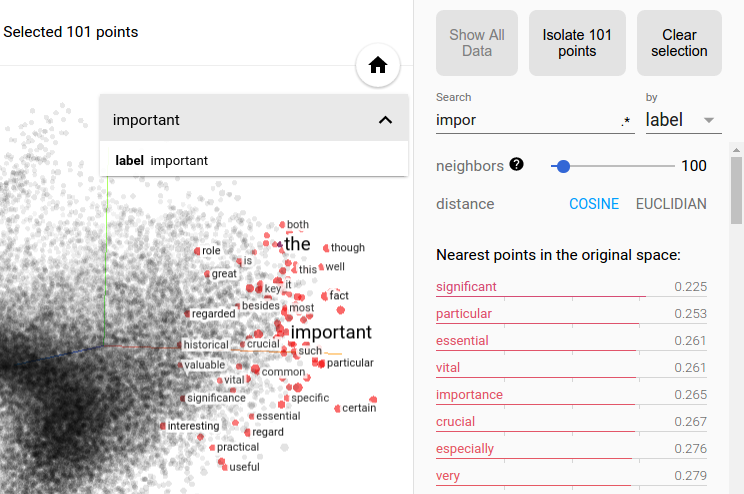
\includegraphics[scale=0.5]{embedding-nearest-points.png}
	\caption{important最相邻的embedding数据集}
\end{figure}
custom projection结合过滤会很有用,下面我们过滤和"politics"100个最相邻的点project他们在x轴上从好到坏向量表示,y轴水机。你可以看右边的我们有"ideas","science","perspective","journalism"左边有"crisis","violence"和"conflict"。
\begin{figure}
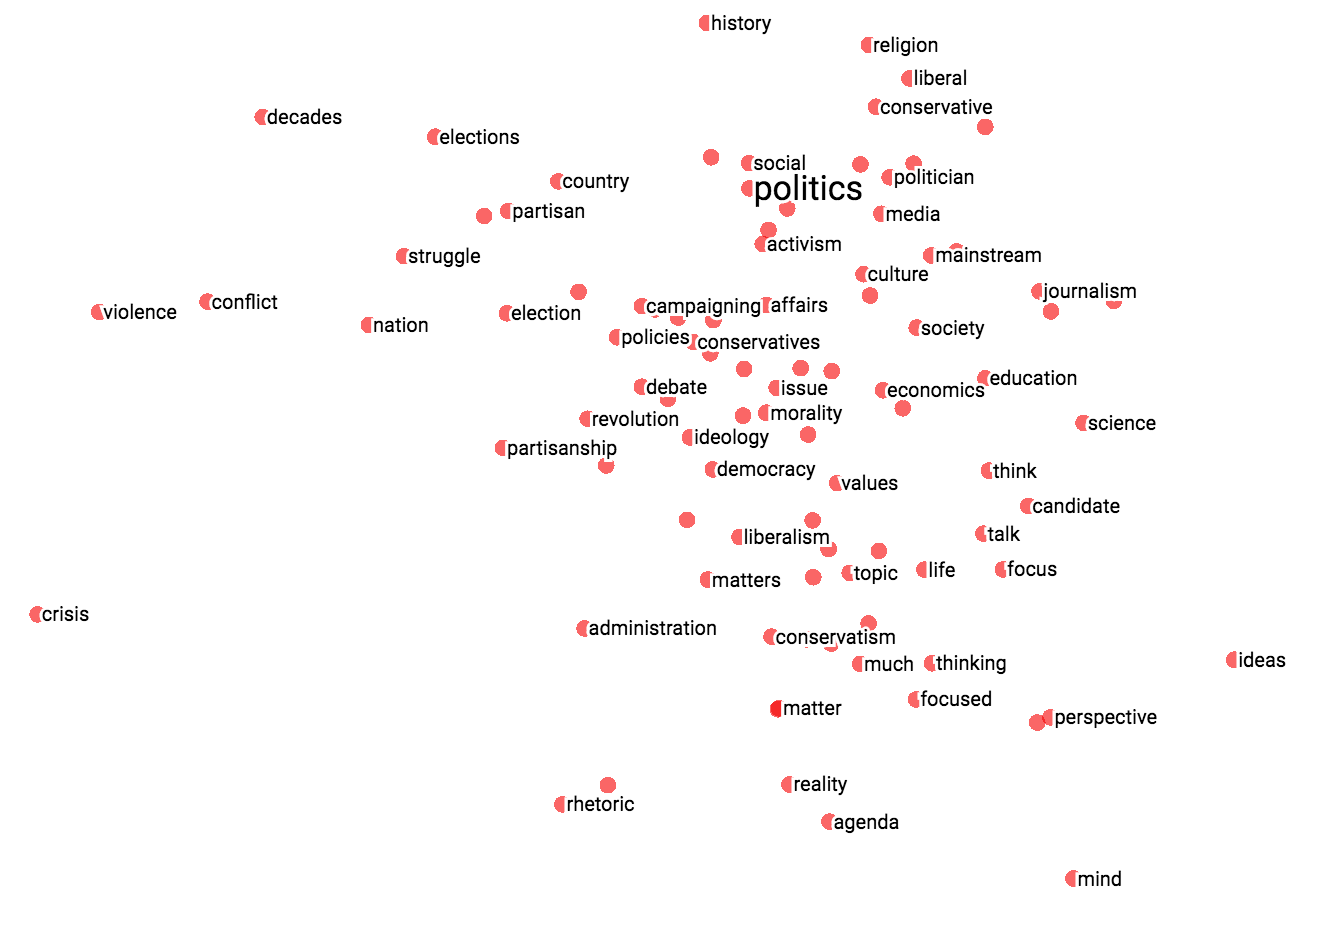
\includegraphics[scale=0.3]{embedding-custom-projection.png}
\end{figure}

\subsection{合作的特性}
为了分享你的发现你可以用右上角的bookmark面板保存当前状态(包括计算任何projection的坐标)为一个小文件。Projector可能被指定到一个或者更多文件,产生下面的面板,其他人可以通过标签序列查看。
\begin{figure}[H]
	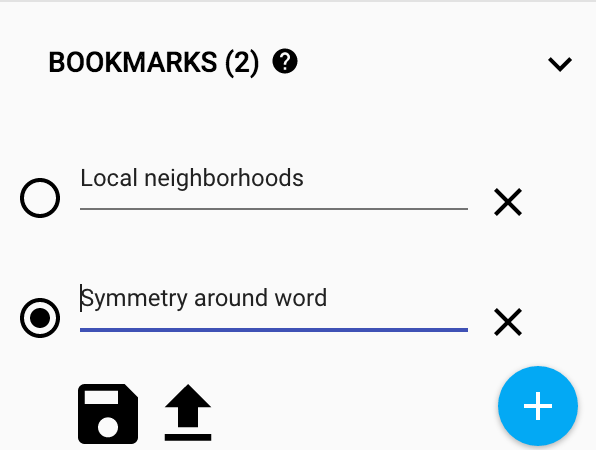
\includegraphics[scale=0.5]{embedding-bookmark.png}
\end{figure}
\subsection{简单的问答}
embedding是一个动作还是一个事物?两者都是,人们谈论向量空间的embedding word形成embedding(事物)。通常两个是一个从离散对象到向量映射embedding概念,创建应用映射是一个行为,但是映射是一个事物。

是高维还是低维embedding?300维的向量字词空间,例如当和上百万的字词空间相比是低维。但是数学上它是高维,显示了大量喝和人们直觉上的2位或者三维空间不一致的特性。

embedding和embedding layer是一样的吗?不是,一个embedding layer是神经网络的一部分,不是一个embedding是一个更常用的概念。
